\chapter{Introducción específica} % Main chapter title

\label{Chapter2}

%----------------------------------------------------------------------------------------
%	SECTION 1
%----------------------------------------------------------------------------------------
En este capítulo se describen los componentes de hardware, el software y los protocolos de comunicación utilizados para el desarrollo del sistema.

\section{Componentes de hardware del sistema}
El sistema está compuesto por un conjunto de componentes electrónicos y módulos que operan de forma coordinada para cumplir las funciones de dispensado, sensado y comunicación. A continuación se describe cada uno de ellos.

\subsection{Microcontrolador STM32F446RE}

El sistema desarrollado incorpora un microcontrolador de 32 bits de la marca STMicroelectronics, modelo F446RE, basado en el núcleo ARM Cortex-M4 con una frecuencia de trabajo de hasta 180 MHz. Dispone de una unidad de punto flotante de precisión simple y memorias embebidas de alta velocidad, entre ellas 512 kB de memoria Flash y 128 kB de SRAM.

Cuenta con un gran número de entradas/salidas, convertidores analógicos-digitales de 12 bits y hasta 17 temporizadores.  Posee además diversas interfaces de comunicación entre las que se destacan UART ({\it{Universal Asynchronous Receiver-Transmitter}}) e I\textsuperscript{2}C ({\it{Inter-Integrated Circuit}}). Para el desarrollo de este trabajo se da uso a la placa de evaluación de la figura \ref{fig:nucleo}, una placa Nucleo de la marca STM modelo F446RE que dispone de todos los periféricos necesarios para el uso del microcontrolador y sus componentes.
\begin{figure}[H]
	\centering
	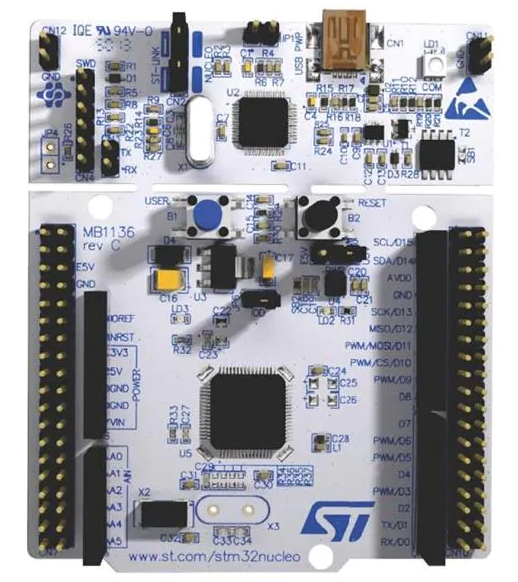
\includegraphics[width=7cm, height=7cm]{./Figures/nucleo.png}
	\caption{Placa de evaluación Nucleo de STM.\protect\footnotemark}
	\label{fig:nucleo}
\end{figure}
\footnotetext{\url{https://www.st.com/en/evaluation-tools/nucleo-f446re.html}}

\subsection{Módulo ESP32}

Para la comunicación inalámbrica con el usuario se utilizó un módulo ESP32, que actúa como puente (\textit{bridge}) entre el microcontrolador STM32 y la aplicación en PC. 
La comunicación entre el STM32 y el ESP32 se realiza a través del protocolo UART, mientras que el ESP32 gestiona la comunicación Bluetooth con la aplicación receptora.

El ESP32 es un SoC (\textit{System on Chip}) desarrollado por Espressif Systems, con doble núcleo Xtensa LX6 a 240 MHz, que integra conectividad Wi-Fi 802.11b/g/n y Bluetooth 4.2 (Classic + BLE (\textit{Bluetooth Low Energy})). 
En este trabajo se utilizó exclusivamente la funcionalidad Bluetooth Classic para la transmisión de datos en formato JSON.

Este microcontrolador fue seleccionado por su compatibilidad con FreeRTOS, la disponibilidad de periféricos I2C y UART necesarios para los módulos del sistema, y la existencia de la placa de evaluación Nucleo-F446RE que simplificó el proceso de prototipado.
 

\subsection{Celda de carga y módulo HX711} 
Para medir el peso del alimento en el plato se utiliza una celda de carga tipo galga extensiométrica combinada con el módulo amplificador y conversor analógico-digital HX711. La celda de carga convierte la fuerza aplicada en una variación de resistencia eléctrica, que el HX711 amplifica y digitaliza con una resolución de 24 bits.

El HX711 se comunica con el microcontrolador mediante una interfaz de dos cables (CLK y DATA) y opera con una tensión de alimentación de 5 V o 3,3 V. Su tasa de muestreo configurable es de 10 o 80 muestras por segundo, lo que resulta suficiente para la aplicación de monitoreo de consumo en intervalos regulares.


\subsection{Motor paso a paso y driver A4988}

El mecanismo de dispensado de alimento fue accionado por un motor paso a paso NEMA 17, seleccionado por su precisión de movimiento y su par motor. Para su control se utilizó el driver A4988 de Pololu, un módulo compacto que permite gestionar motores paso a paso bipolares con corrientes de hasta 2 A por fase.

El driver A4988 acepta señales de dirección (DIR) y paso (STEP) provenientes del microcontrolador, y permite seleccionar la resolución de micropasos (full, 1/2, 1/4, 1/8 y 1/16) mediante pines de configuración. Su tensión de alimentación lógica es de 3,3 V a 5,5 V, mientras que la tensión de potencia puede ser de hasta 35 V.

\subsection{Módulo RTC DS3231}

Para la gestión autónoma de los horarios de dispensado se incorporó un módulo de reloj de tiempo real (RTC) basado en el integrado DS3231 de Maxim Integrated. Este dispositivo proporciona información de fecha y hora con una precisión de ±2 ppm, equivalente a aproximadamente 1 minuto de desviación por año.

El DS3231 se comunica con el microcontrolador mediante el protocolo I2C y dispone de una batería de respaldo (batería de litio tipo botón CR2032) que mantiene el funcionamiento del reloj ante cortes de energía. Incorpora además un sensor de temperatura interno para la compensación de la oscilación del cristal, lo que contribuye a su alta precisión.

\subsection{Pulsador de dispensado manual}
El sistema incorpora un pulsador físico que permite al usuario activar el dispensado de alimento de forma manual, fuera de los horarios programados. Este componente se conecta directamente a un pin de entrada digital del microcontrolador con resistencia de pull-up interna habilitada por software. La detección de la pulsación se realizó mediante interrupción externa, lo que garantiza una respuesta inmediata independientemente de las tareas en ejecución.

\section{Software y entorno de desarrollo}

\subsection{STM32CubeIDE}

STM32CubeIDE es un entorno de desarrollo integrado (IDE) de código abierto para programar microcontroladores y microprocesadores de la familia STM32. Basado en Eclipse, permite configurar periféricos, generar código inicial de forma automática, compilar y depurar en la misma plataforma. Se utilizó en este trabajo para el desarrollo completo del firmware del STM32.

\subsection{FreeRTOS}

FreeRTOS es un sistema operativo de tiempo real (RTOS) de código abierto ampliamente utilizado en sistemas embebidos. Provee mecanismos de planificación de tareas, semáforos, colas de mensajes y temporizadores de software que facilitan la gestión de múltiples procesos concurrentes. En este trabajo, FreeRTOS se integró como \textit{middleware} sobre la capa de abstracción de hardware (HAL) del STM32, y es utilizado para gestionar las tareas de lectura de sensores, control del motor, comunicación UART y manejo del pulsador.

\subsection{Arduino IDE / ESP-IDF (ESP32)}

Para el desarrollo del firmware del módulo ESP32 se utilizó el entorno Arduino IDE con soporte para la plataforma ESP32. Este entorno simplifica el acceso a las bibliotecas de comunicación Bluetooth Classic (SPP - Serial Port Profile), que permiten establecer una conexión serie inalámbrica entre el ESP32 y la aplicación en PC.

\subsection{Lenguaje de programación C}

El firmware del microcontrolador STM32 se desarrolla íntegramente en lenguaje C, un lenguaje de propósito general que permite el control directo del hardware y la gestión eficiente de los recursos del sistema. Su portabilidad y compatibilidad con las bibliotecas HAL de STM32 y con FreeRTOS lo convirtieron en la opción más adecuada para este tipo de desarrollo.

\section{Protocolos de comunicación}

El sistema desarrollado hace uso de tres protocolos de comunicación para la transferencia de datos entre el microcontrolador y los distintos módulos que lo componen.

\subsection{Protocolo I2C}

Se emplea el protocolo I2C para la comunicación entre el microcontrolador y el módulo RTC DS3231. Este protocolo consiste en un bus serie síncrono, bidireccional y semidúplex, organizado bajo una arquitectura maestro-esclavo. Utiliza dos líneas eléctricas: SCL para la señal de reloj y SDA para la transferencia de datos. La comunicación se basa en tramas que incluyen la dirección de 7 bits del dispositivo, un bit de lectura/escritura y un mecanismo de confirmación mediante señales ACK y NACK.

\subsection{Protocolo UART}

El protocolo UART se utiliza para la comunicación serie entre el microcontrolador STM32 y el módulo ESP32. UART es un protocolo asíncrono que utiliza dos líneas físicas: una de transmisión (TX) y otra de recepción (RX). Los datos se transmiten en tramas compuestas por un bit de inicio, los bits de datos (generalmente 8) y un bit de parada. En este sistema se configuran ambos extremos con una velocidad de 115200 baudios, sin paridad y con un bit de parada.

\subsection{Bluetooth Classic (SPP)}

El módulo ESP32 gestiona la comunicación inalámbrica con la aplicación en PC mediante Bluetooth Classic bajo el perfil SPP (Serial Port Profile). Este perfil emula una comunicación serie sobre el canal Bluetooth, lo que facilita la integración con el microcontrolador, ya que el ESP32 recibe datos por UART desde el STM32 y los reenvía por Bluetooth, y viceversa. Los datos se transmiten en formato JSON, lo que permite estructurar la información de manera legible y extensible.